\section{Moir\'e as a field}
\label{sec:field}

\subsection{A layer is two scalar fields}

\begin{definition}[Family]
A \emph{family} is a countable collection of curves $\{\gamma_n\}_{n\in\Z}$ in
$\R^2$, together with an index convention that names them.
\end{definition}

We never represent $\{\gamma_n\}$ as geometry. A layer is represented by two
functions of a continuous position $p\in\R^2$:
\begin{align}
  \idx(p) &\in \R && \text{the \emph{index field}: } \gamma_n=\idx^{-1}(n),\\
  d(p) &= \min_{n} \mathrm{dist}(p,\gamma_n) && \text{the \emph{distance field}.}
\end{align}
The index field is fractional --- $\idx(p)=7.3$ means $p$ lies three tenths of the
way from member $7$ to member $8$. The distance field is Euclidean and unsigned.

Most families in practice are the level sets of a single scalar \emph{phase}
function. It is convenient to keep the phase in world units, so that member $n$ is
the level set $\{\ph = ns + \varphi\}$ with $s$ the spacing and $\varphi$ an
offset. Then
\begin{equation}
  \idx(p) = \frac{\ph(p)-\varphi}{s},
  \qquad
  d(p) \;\simeq\; \frac{\mathrm{pd}\!\left(\ph(p)-\varphi,\; s\right)}{\lVert\nabla\ph(p)\rVert},
  \label{eq:eikonal}
\end{equation}
where $\mathrm{pd}(v,s)=\min_{k\in\Z}|v-ks|$ is the distance from $v$ to the
lattice $s\Z$. Both are one line of shader code.

\subsection{The gradient is not optional}
\label{sec:eikonal}

\begin{figure}[t]
  \centering
  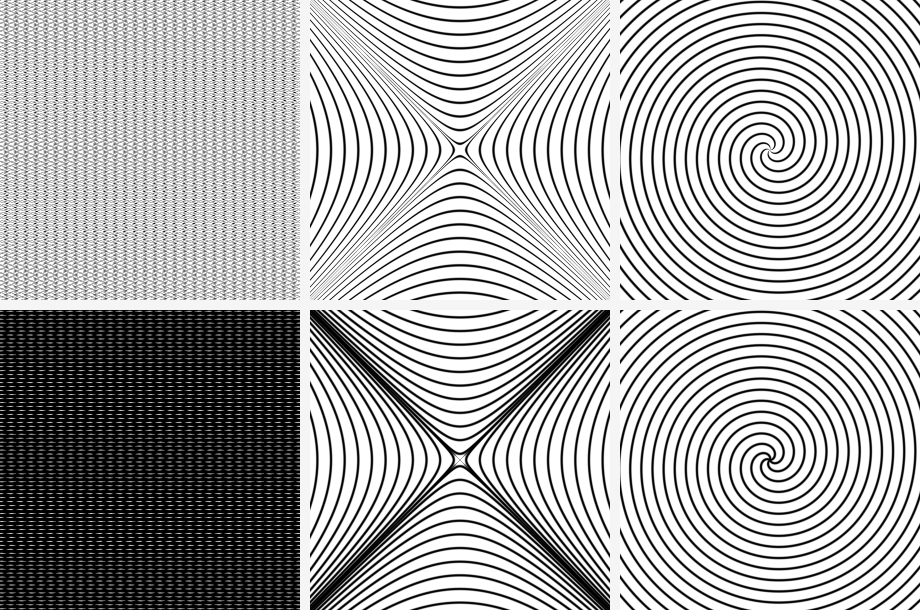
\includegraphics[width=\linewidth]{figures/gradient-compare.png}
  \panelrow{0.32609}{0.01087}{wave, hyperbola, spiral}
  \Description{A two-by-three grid of black-on-white panels: a wave family, a
  hyperbola family and a spiral family, drawn twice. In the top row the strokes fade
  to nothing towards the edges where the curves crowd together; in the bottom row
  those same regions are solid black.}
  \caption{\figlead{A phase residual is not a distance.} Top: what our shader drew
  for the wave, hyperbola and spiral families --- the phase residual, undivided.
  Strokes thin by exactly the factor the family is steep by, so the pattern fades
  where it should saturate and the hyperbola's asymptotes disappear. Bottom: the
  same settings with Eq.~\ref{eq:eikonal}. The parabola family always divided; these
  three did not, and the failure is worst exactly where the family is densest.}
  \label{fig:gradient}
\end{figure}

The division by $\lVert\nabla\ph\rVert$ in Eq.~\ref{eq:eikonal} converts a phase
residual into a length. It is easy to omit, and we omitted it. Our shader applied
it for the parabola family and not for the wave, hyperbola or spiral, with two
consequences.

The first is cosmetic but severe. Where $\lVert\nabla\ph\rVert=g>1$, the reported
distance is $g$ times too large, so the stroke is $g$ times too thin. Sweeping each
family over its own slider range on a $1400\times880$ frame
(Appendix~\ref{app:atlas}, Table~\ref{tab:gradient}) we measure $g$ up to
$\gradWorstWave$ for the wave and $\gradWorstHyp$ for the hyperbola, with more than
half the frame off by over $10\%$ in both cases. Visually the family pales out
exactly where it steepens and crowds --- the opposite of what the geometry does
(Figure~\ref{fig:gradient}).

The second is a correctness bug. Our stroke half-width is
$\mathrm{halfT}=\max(t/2,\,1.15\,\mathrm{px})$, and the floor exists so that a
hairline stays a hairline instead of breaking into speckle when zoomed out
(Section~\ref{sec:zoom}). That floor is a statement about \emph{screen} distance.
Compared against an undivided phase residual it is a statement about phase, and it
guarantees nothing wherever $g\neq1$. The families that most need the floor --- the
steep ones --- are precisely the ones that were not getting it.

We adopt Eq.~\ref{eq:eikonal} everywhere. One honest cost: a wave at high amplitude
and frequency now saturates to solid ink, because at those settings its members
genuinely are closer together than a stroke width. That is the correct answer, and
the previous behaviour was hiding it.

Eq.~\ref{eq:eikonal} is an eikonal approximation and it is exact only where the
family is locally a foliation with steady gradient. The one family in our
catalogue that violates this is the hyperbola, whose level sets cross on its
asymptote cross; we return to it in Section~\ref{sec:limits}.

\subsection{Compositing}

Layers composite as ink over paper. With stroke half-width $h_i$ and antialias
band $a$, layer $i$ contributes coverage
\begin{equation}
  \alpha_i(p) = \Big(1-\mathrm{smoothstep}(h_i-a,\;h_i+a,\;d_i(p))\Big)\,o_i,
  \label{eq:alpha}
\end{equation}
and the frame is the running \texttt{mix} of background with each layer's colour
at that alpha. For two black layers on white this is the union
$\alpha_1+\alpha_2-\alpha_1\alpha_2$. There is no separate composite pass, no
intermediate texture, and no place in the pipeline where a layer exists as pixels.

Three properties follow immediately and are the practical reason to do it this way.

\emph{No resolution.} $\idx$ and $d$ are defined at every real position, so
changing zoom changes only where they are sampled. A moir\'e authored at one scale
is the same moir\'e at another (Section~\ref{sec:zoom}).

\emph{Bounded frequency by construction.} The stroke floor
$h\ge1.15\,\mathrm{px}$ means the ink field's transition band is never narrower
than a pixel, so the composite is band-limited without any filtering step. This is
the thing the suppression literature achieves with prefiltering and the synthesis
literature cannot achieve at all: we get to keep the designed difference component
and lose the undesigned ones, because the undesigned ones are never created.

\emph{Editability.} Every parameter enters $\idx$ and $d$ analytically. Moving a
slider does not invalidate a cached raster, because there is none.

\subsection{The fringe law}
\label{sec:fringe}

Now the observation the rest of the paper rests on. Superpose two layers. Where
does the visible pattern come from?

Fix a point $p$ and let $D=\idx_1-\idx_2$ be the difference of index fields. Write
$w_i$ for layer $i$'s stroke half-width measured \emph{in index units},
$w_i=h_i\lVert\nabla\idx_i\rVert$, and $b_i=a\lVert\nabla\idx_i\rVert$ for its
band. Define the index-space stroke profile
$A_i(u)=1-\mathrm{smoothstep}(w_i-b_i,\,w_i+b_i,\,\mathrm{pd}(u,1))$.

\begin{theorem}[Fringe law]
\label{thm:fringe}
Let $u$ be the direction of the mean index gradient
$g=\tfrac12(\nabla\idx_1+\nabla\idx_2)$, let $T=1/\lVert g\rVert$ be the carrier
period, and let $S=p+[-T/2,T/2]\,u$. Suppose that on $S$ both families are local
foliations and that $D$ is constant. Then the mean ink over $S$ is
\begin{equation}
  \label{eq:phi}
  \begin{gathered}
    \bar\alpha(p) \;=\; \Phi\big(D(p)\big), \qquad\text{where}\\
    \Phi(g) \;=\; \int_0^1 \Big[A_1(v)+A_2(v-g)-A_1(v)A_2(v-g)\Big]\,\mathrm{d}v,
  \end{gathered}
\end{equation}
which depends on $p$ only through $D(p)$. If instead $D$ is merely affine on $S$,
the same expression holds up to an error $O(\het)$ in the ratio \eqref{eq:ratio}
below. In the hard-edged limit $b_i\to0$,
\begin{equation}
  \Phi(g) = 2w_1+2w_2-\max\!\big(0,\;w_1+w_2-\mathrm{pd}(g,1)\big):
  \label{eq:tent}
\end{equation}
a tent in $D$, rising from $2\max(w_1,w_2)$ at $D\in\Z$ to a plateau of
$2w_1+2w_2$ once the strokes clear each other.
\end{theorem}

The proof is a change of variables and is given in Appendix~\ref{app:fringe}; the
content is entirely in the statement. It is worth being exact about the two
hypotheses, because they are not interchangeable. ``Both families are local
foliations on $S$'' is what lets us reparameterise the segment by index instead of
by arclength. ``$D$ is constant on $S$'' is what makes the answer a function of
$D(p)$ alone, and it is the strong one: exact constancy means the two carriers
agree exactly in pitch and direction, so the interesting cases only satisfy it
approximately. The appendix carries the affine case through and shows the
correction is first order in $\het$, which is the same small parameter
\S\ref{sec:visibility} uses to decide whether a fringe exists at all. So the
theorem is exact in the limit that a fringe becomes infinitely broad, and
degrades in the parameter that measures how far from that limit we are --- which is
why the verification below both restricts to $\het\le1/4$ and reports the residual
rather than claiming zero. Three further things are worth saying.

\paragraph{The locus is classical; the profile is not.}
$\Phi$ is periodic with period $1$ and extremal at $D\in\Z$ and
$D\in\Z+\tfrac12$. So the light fringes are exactly $\{D\in\Z\}$ --- where the two
families' members locally coincide and their strokes overlap, wasting ink --- and
the dark fringes are exactly $\{D\in\Z+\tfrac12\}$, where the members interleave
and the ink is maximally spread. \textbf{The moir\'e is the contour plot of
$\idx_1-\idx_2$ at unit interval.} Nothing else about either family survives the
average.

That locus is not ours and we want to be exact about whose it is. Writing the two
families as $\idx_1=m$, $\idx_2=n$ and asking where their members cross in a fixed
relation $m-n=k$ is the \emph{indicial equation}, which is how Oster, Wasserman and
Zwerling read moir\'e in 1964~\cite{Oster1964} and how Amidror presents the
geometric approach~\cite{Amidror2009Theory}; the same relation, read backwards, is
the fringe-order law of moir\'e
interferometry~\cite{Post2008Moire}. If the reader's summary of
Theorem~\ref{thm:fringe} is ``the fringes are the unit level sets of the index
difference'', they have learned nothing after 1964, and should stop there.

What the theorem adds is everything to the left of the locus. The classical
argument identifies a set of curves; it does not say what \emph{value} the frame
takes between them, and a renderer has to produce that value at every pixel. $\Phi$
does: it is the mean coverage of the actual compositing operator
(Eq.~\ref{eq:alpha}), so it carries the stroke widths, the saturation, and the
antialias band, and it holds where nothing is periodic, where the two carriers are
different families, and per-pixel rather than in the asymptotic limit of a
grating pair. It comes with $\het$ (\S\ref{sec:visibility}), which says where it
may be trusted --- the classical accounts assume the near-matched regime rather
than measuring it. And because it is a formula for averaged ink rather than a set
of curves, it can be \emph{drawn} (\S\ref{sec:envelope}) and it can be
\emph{inverted} (\S\ref{sec:beyond}). Those are the parts we lean on.

\paragraph{It is a tent, not a sinusoid, and it saturates.}
Grating models built on the first Fourier component predict a sinusoidal fringe
profile. Eq.~\ref{eq:tent} says the profile is piecewise linear with a flat top,
and the flat top is reached as soon as $\mathrm{pd}(D,1)>w_1+w_2$. This is why
field-composited moir\'e looks crisper than the same pattern built spectrally: most
of the fringe is at full contrast, and the transition occupies only a
$(w_1{+}w_2)$-wide sliver of each period. It also explains a design behaviour we
had noticed but not understood --- past a certain stroke thickness, thickening the
strokes stops changing the fringe and only darkens the whole frame.

\paragraph{No periodicity is required.}
$\idx_1$ and $\idx_2$ are arbitrary. The theorem's hypotheses are local
(affineness of $D$ over one carrier period, and the eikonal condition) and say
nothing about global structure. A spiral is admissible. Two hyperbola families are
admissible. A pencil of rings each rotated by $n\theta$, which is not a geometric
transform of any periodic layer, is admissible.

\subsection{The envelope view}
\label{sec:envelope}

$\bar\alpha$ is a quantity, so it can be drawn, and drawing it gives the author
the fringe system with the carrier removed. The obvious way to get such a picture
is to blur the render, and it is the wrong way: a blur is a kernel in pixels, so
it changes under zoom, it softens every real edge along with the carrier, and its
width has to be retuned whenever the pitch changes.

Look again at the hypothesis of Theorem~\ref{thm:fringe}. Over the averaging
segment every family's index advances by the \emph{same} amount --- that is what
$D$ constant means --- so the entire stack is a one-parameter object. Advance every
layer's index together by $u$ and average over $u\in[0,1)$:
\begin{equation}
  \bar\alpha(p) \;=\; \int_0^1 \alpha\big(p;\; \idx_i \mapsto \idx_i + u\big)\,\mathrm{d}u.
  \label{eq:meanink}
\end{equation}
This is an average over \emph{index}, not over space. No sample is taken off
centre, so nothing is blurred; the result is the theorem's own $\bar\alpha$ at the
full resolution of the frame, and it is identical at every zoom. Since the
integrand is periodic in $u$ with period exactly $1$, a uniform grid of $M$ nodes
is exact but for harmonics above $M$; the integrand is a composite of trapezoids,
so $M=\envTaps$ leaves an error far below one colour step. Every ``averaged ink''
panel in this paper is \eqref{eq:meanink} at $M=\envTaps$, and it is a toggle in
the Studio, not a post-process.

Written that way, \eqref{eq:meanink} is an integral over the diagonal of the
\emph{index torus} $[0,1)^K$ --- one circle per family --- and the choice of the
diagonal is exactly Theorem~\ref{thm:fringe}'s hypothesis rather than a
convenience. It is worth saying what the honest alternative is, because we
implemented it first. Sweeping a rigid translation of the whole stack is
geometrically exact where advancing an index is bookkeeping, and it is unusable:
the taps then sample a two-dimensional disc for strokes that cover a few percent
of it, so a handful of taps carry the answer and the rest carry noise. Sixty-four
of them left the carrier standing and the fringes mottled. The diagonal's fiction
is what makes it exact.

\paragraph{One solve, many taps.}
The cost, done naively, is $M$ full evaluations of every layer --- and for a
walking family one evaluation is the search of \S\ref{sec:inverse}, so $\envTaps$
of them per pixel is not a view, it is a stall. It was: our first envelope ran at
five frames a second on the tool's own opening preset.

It need not, and the reason is that advancing an index by less than one does not
change \emph{which} members are nearby. So the solver is asked once per pixel for
a \emph{phase sample}
\begin{equation}
  \Pi(p) \;=\; \big(\,\rho,\; \rho^{\uparrow},\; \rho^{\downarrow},\; \ell\,\big),
  \label{eq:phasesample}
\end{equation}
the signed distances to the nearest member and to the two flanking it, together
with a floor $\ell$ that does not participate. A tap at $u$ then reads
\begin{equation}
  d(p;u) \;=\; \max\Big(\min_{k\in\{\rho,\rho^{\uparrow},\rho^{\downarrow}\}} \lvert k - u\,g \rvert,\; \ell\Big),
  \label{eq:slide}
\end{equation}
where $g=\lvert\rho^{\uparrow}-\rho\rvert$ is the \emph{local} member gap. Because
the sweep is centred on $u=0$, the triple brackets every phase it visits, so
\eqref{eq:slide} is not an approximation of the re-solved distance --- it is that
distance, in nine instructions. The search runs once per pixel and the sweep is
arithmetic. Median frame times in the envelope view went from hundreds of
milliseconds to inside the frame.

Two things fall out of writing the sample this way. The gap $g$ is local, so a
tap covers exactly one period of \emph{this} family at \emph{this} point, whatever
the pitch does across the frame --- which is what the radial pencil needs, since
its member gap $2r\sin(\pi/2N)$ grows with radius. And $\ell$ is where the
non-sliding parts of a family live: the guard returned by a saturated solve, the
hole at the centre of a pencil, the missing inner neighbour of the innermost
hyperbola. Those are the places where there is genuinely nothing to slide onto,
and separating them from the residual is what keeps the average from inventing
ink there.

\paragraph{Every family has a currency.}
Equation~\ref{eq:meanink} advances an index, and each family spends that in its
own coin. The level-set families of \S\ref{sec:catalog} shift a phase. The radial
pencil turns: advancing its index by $u$ rotates the fan by $u\pi/N$, which is
how a family whose index is an angle joins an average built for scalars. A lattice
indexes its members by a \emph{pair} of integers, so it translates along its two
generators --- and here the diagonal is exactly wrong. Stepping both generators in
lockstep keeps their two indices correlated, and a lattice then beats against
itself: a fine diagonal hatch at the carrier's own scale that no amount of
contrast can be read through. So we take the $i$th tap along the first generator
to $u_i$ and along the second to $\{i\varphi\}$, $\varphi$ the golden ratio ---
the Fibonacci lattice, a rank-1 rule on the
two-torus~\cite{Sloan1994Lattice, Keller2013Quasi}. It decorrelates a lattice from
itself while leaving it in step with every other layer's matching generator, which
is where the fringes an author wants actually are.

\paragraph{A pivot, not a gain.}
The view exposes a contrast, because a fringe field is a small excursion about the
stack's mean coverage and the interesting part is the excursion. Expanding about
$0$ would ride the mean up and down as the fringes move, so the expansion is about
the coverage the stack would average over its own periods: $2h/s$ per family,
composited. Counting a lattice's families is not optional. A hex lattice draws
three, and calling its coverage that of one puts the pivot far brighter than the
picture it is expanding about, which at any real contrast drives the whole frame
black --- which is precisely how we found the bug.

One caveat remains, and it is structural rather than a matter of implementation.
The average is over the diagonal, so where Theorem~\ref{thm:fringe}'s hypothesis
fails --- where $\het$ is large --- the view still shows $\Phi(D)$ faithfully, but
$\Phi(D)$ is no longer what the eye will average. The honest reading of the two
together is the ratio map beside the envelope.

\subsection{When is there a fringe at all?}
\label{sec:visibility}

Theorem~\ref{thm:fringe} needs $D$ to be nearly constant over one carrier period.
Both requirements are about the same ratio. Define the \emph{heterodyne ratio}
\begin{equation}
  \het(p) = \frac{\lVert\nabla D(p)\rVert}{\lVert g(p)\rVert}
  = \frac{\lVert\nabla\idx_1-\nabla\idx_2\rVert}
         {\big\lVert\tfrac12(\nabla\idx_1+\nabla\idx_2)\big\rVert}.
  \label{eq:ratio}
\end{equation}
$D$ changes by $\het$ across one carrier period, so $\het\ll1$ is exactly the
condition that a fringe be large compared with the carrier. It is the field-space
form of the classical requirement that the two frequencies be close --- and it is a
\emph{field}, so it varies over the frame, and it can be drawn
(Figure~\ref{fig:visibility}).

\begin{figure*}[t]
  \centering
  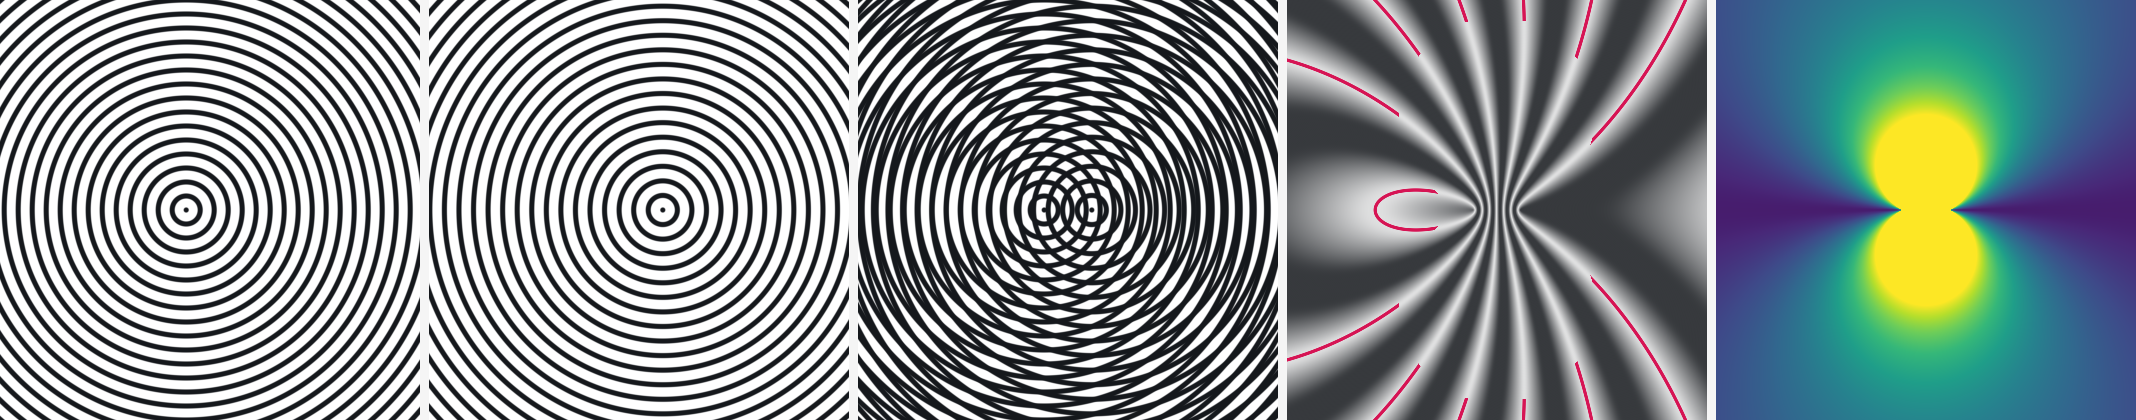
\includegraphics[width=\linewidth]{figures/fringe-law.png}
  \panelrow{0.19663}{0.00421}{%
    (a) layer $1$,
    (b) layer $2$,
    (c) superposition,
    (d) averaged ink\, $+\;\{D\in\Z\}$,
    (e) heterodyne ratio $\het$}
  \Description{Five square panels. The first two are black-on-white concentric rings
  about slightly different centres. The third overlays them and shows large curved
  bands cutting across the rings. The fourth is a smooth grey field of broad light
  and dark bands fanning out from the centre, its light bands traced by thin crimson
  curves that stop short of two blank lobes either side of centre. The fifth is a
  blue-to-yellow heat map of the same frame, dark blue over most of it with two
  bright yellow lobes where the crimson curves stopped.}
  \caption{\figlead{The moir\'e is a contour plot of the index difference.}
  \textbf{(a,\,b)} Two circle families, rendered alone from their own distance
  fields. Their centres differ by $34$ units and their pitches by four percent, and
  nothing else. \textbf{(c)} Their superposition, in which a fringe system appears
  that is in neither layer. \textbf{(d)} The theorem is a statement about averaged
  ink, so this is that average: the envelope view of \S\ref{sec:envelope}, which
  integrates the same two fields over one period of their common phase and so
  removes the carriers without blurring anything --- with the unit level sets of
  $D=\idx_1-\idx_2$ laid over it in crimson. Those curves are computed from the two
  index fields alone and never from the image, and they land on the light fringes.
  They are drawn only where
  $\het\le1/4$, which is why they stop short of the two lobes flanking the centres.
  \textbf{(e)} The heterodyne ratio $\het$ of Eq.~\ref{eq:ratio} over the same
  frame, dark where Theorem~\ref{thm:fringe} applies and bright where the two
  carriers are too different for a fringe to exist. The bright lobes are exactly the
  region the overlay declines to describe, and in the superposition they are exactly
  the region that reads as a rosette of crossings rather than as bands.}
  \label{fig:visibility}
\end{figure*}

We take $\het\le1/4$ as the operational definition of the fringe regime.

\subsection{Verification}

Theorem~\ref{thm:fringe} is a claim about a rendered image, so we measured it.
For ten scene pairs spanning straight, curved, isotropic, anisotropic, periodic and
aperiodic families, we compute the exact one-period directional mean of the union
from the fields themselves --- no raster, so no sampler error --- and compare it
against $\Phi$ evaluated at the window centre. There is no fitting and no free
parameter. Points are excluded on three stated grounds: strokes merged
($w_i+b_i>0.45$, so no gaps remain to beat), carrier bending more than $0.15$\,rad
across its own period, and gradient varying more than $15\%$ across a period, which
is the eikonal condition of Section~\ref{sec:eikonal}.

% GENERATED by paper/tools/numbers.mjs
\begin{table*}[t]
\caption{\figlead{The fringe law, measured.} Mean and $99$th-percentile absolute
error between the one-period directional mean of the rendered ink and $\Phi(D)$ of
Eq.~\ref{eq:phi}, over samples in the fringe regime $\het\le1/4$. \emph{Swing} is
the range of measured coverage, so it says how much fringe there was to get wrong.
\emph{Light\,/\,dark} are the mean distances of the measured lightest and darkest
deciles from the nearest integer index difference; the ideals are $0$ (light
fringes at $D\in\Z$) and $0.5$ (dark fringes at $D\in\Z+\tfrac12$). Where the
profile plateaus (low swing), the darkest decile spreads across the flat top and
its mean falls short of $0.5$ by construction. \emph{In regime} is the share of admissible samples with $\het\le1/4$. The
last row has none: with those settings no fringe exists, and the criterion says so
without rendering.}
\label{tab:fringe}
% The Families column carries long prose; \small leaves the widest row 11pt
% over the full text width, which prints into the margin.
\footnotesize
\centering
\begin{tabular}{@{}llrrrrcr@{}}
\toprule
Scene & Families & $n$ & mean & p99 & swing & light\,/\,dark & in regime \\
\midrule
\texttt{parallel-rotate} & two line families 6 degrees apart & 14,641 & 0.0000 & 0.0000 & 0.320 & 0.024 / 0.474 & 100\% \\
\texttt{parallel-pitch} & same direction, pitch mismatched by 4 percent & 14,641 & 0.0059 & 0.0189 & 0.326 & 0.026 / 0.470 & 100\% \\
\texttt{circle-circle} & circle families with displaced centres & 6,118 & 0.0000 & 0.0001 & 0.277 & 0.028 / 0.465 & 45\% \\
\texttt{circle-parallel} & circles under lines; D is not periodic in p & 3,952 & 0.0000 & 0.0000 & 0.242 & 0.034 / 0.475 & 27\% \\
\texttt{hexagon-hexagon} & anisotropic metric, hexagons 4 degrees apart & 13,382 & 0.0000 & 0.0000 & 0.260 & 0.024 / 0.475 & 95\% \\
\texttt{square-circle} & two different norms at the same spacing & 3,524 & 0.0000 & 0.0001 & 0.242 & 0.002 / 0.460 & 25\% \\
\texttt{spiral-circle} & aperiodic family: Archimedean spiral over circles & 14,041 & 0.0000 & 0.0001 & 0.243 & 0.031 / 0.461 & 100\% \\
\texttt{parabola-parabola} & curved families, bend mismatched by 8 percent & 484 & 0.0166 & 0.0329 & 0.169 & 0.160 / 0.218 & 100\% \\
\texttt{wave-parallel} & a wave family over lines & 14,641 & 0.0003 & 0.0011 & 0.118 & 0.011 / 0.170 & 100\% \\
\texttt{hyperbola-hyperbola} & rectangular hyperbolae, spacing mismatched by 4 percent & 11,036 & 0.0079 & 0.0214 & 0.640 & 0.123 / 0.430 & 100\% \\
\texttt{walking-circle} & a walking family (member $n$ displaced by $n\delta$) over concentric circles & 11,231 & 0.0159 & 0.0731 & 0.388 & 0.037 / 0.403 & 82\% \\
hyperbola\hspace{0.5pt}-\hspace{0.5pt}parallel & hyperbolae under lines: almost no fringe regime exists & --- & --- & --- & --- & --- & $0$ \\
\bottomrule
\end{tabular}
\end{table*}


Table~\ref{tab:fringe} reports the result. Across $\fringeSamples$ admissible
in-regime samples the mean absolute coverage error is $\fringeMeanErr$ and the
worst $99$th percentile over any scene is $\fringeWorstP$, against a fringe swing of
$0.24$--$0.64$ in coverage. The measured light fringes sit at mean index-gap
$\fringeLight$ from an integer and the dark fringes at $\fringeDark$ from a
half-integer, against ideals of $0$ and $0.5$.

The last row is the informative one. \texttt{hyperbola-parallel} has \emph{no}
in-regime samples anywhere in the frame: $\het>1/4$ everywhere, because a hyperbola
family's index gradient sweeps through all directions while a line family's does
not. There is no fringe in that superposition, only a lattice of crossings, and the
theory says so before rendering.
